\subsubsection{Xây dựng kịch bản video}

Một trong những tính năng nổi bật của hệ thống Smart Gallery là khả năng tạo video slideshow tự động từ bộ sưu tập ảnh. Để thực hiện điều này, hệ thống cần xây dựng một kịch bản video có cấu trúc hợp lý, đảm bảo nội dung mạch lạc và hấp dẫn. Kịch bản video được chia thành bốn phần chính:

\begin{enumerate}
    \item \textbf{Intro:}\newline
    Phần mở đầu của video bao gồm 1 slide tiêu đề và 1 slide tổng quát. Slide tiêu đề sẽ hiển thị tên video do người dùng đặt, trong khi slide tổng quát sẽ giới thiệu nội dung chính của video bằng các hình ảnh đại diện được chọn lọc từ bộ ảnh input của người dùng.
    
    \begin{figure}[H]
        \centering
        \begin{subfigure}{0.48\textwidth}
            \includegraphics[width=1\linewidth]{figures/c4/4_1/intro_1.png} 
            \caption{Slide tiêu đề video.}
        \end{subfigure}
        \hfill
        \begin{subfigure}{0.48\textwidth}
            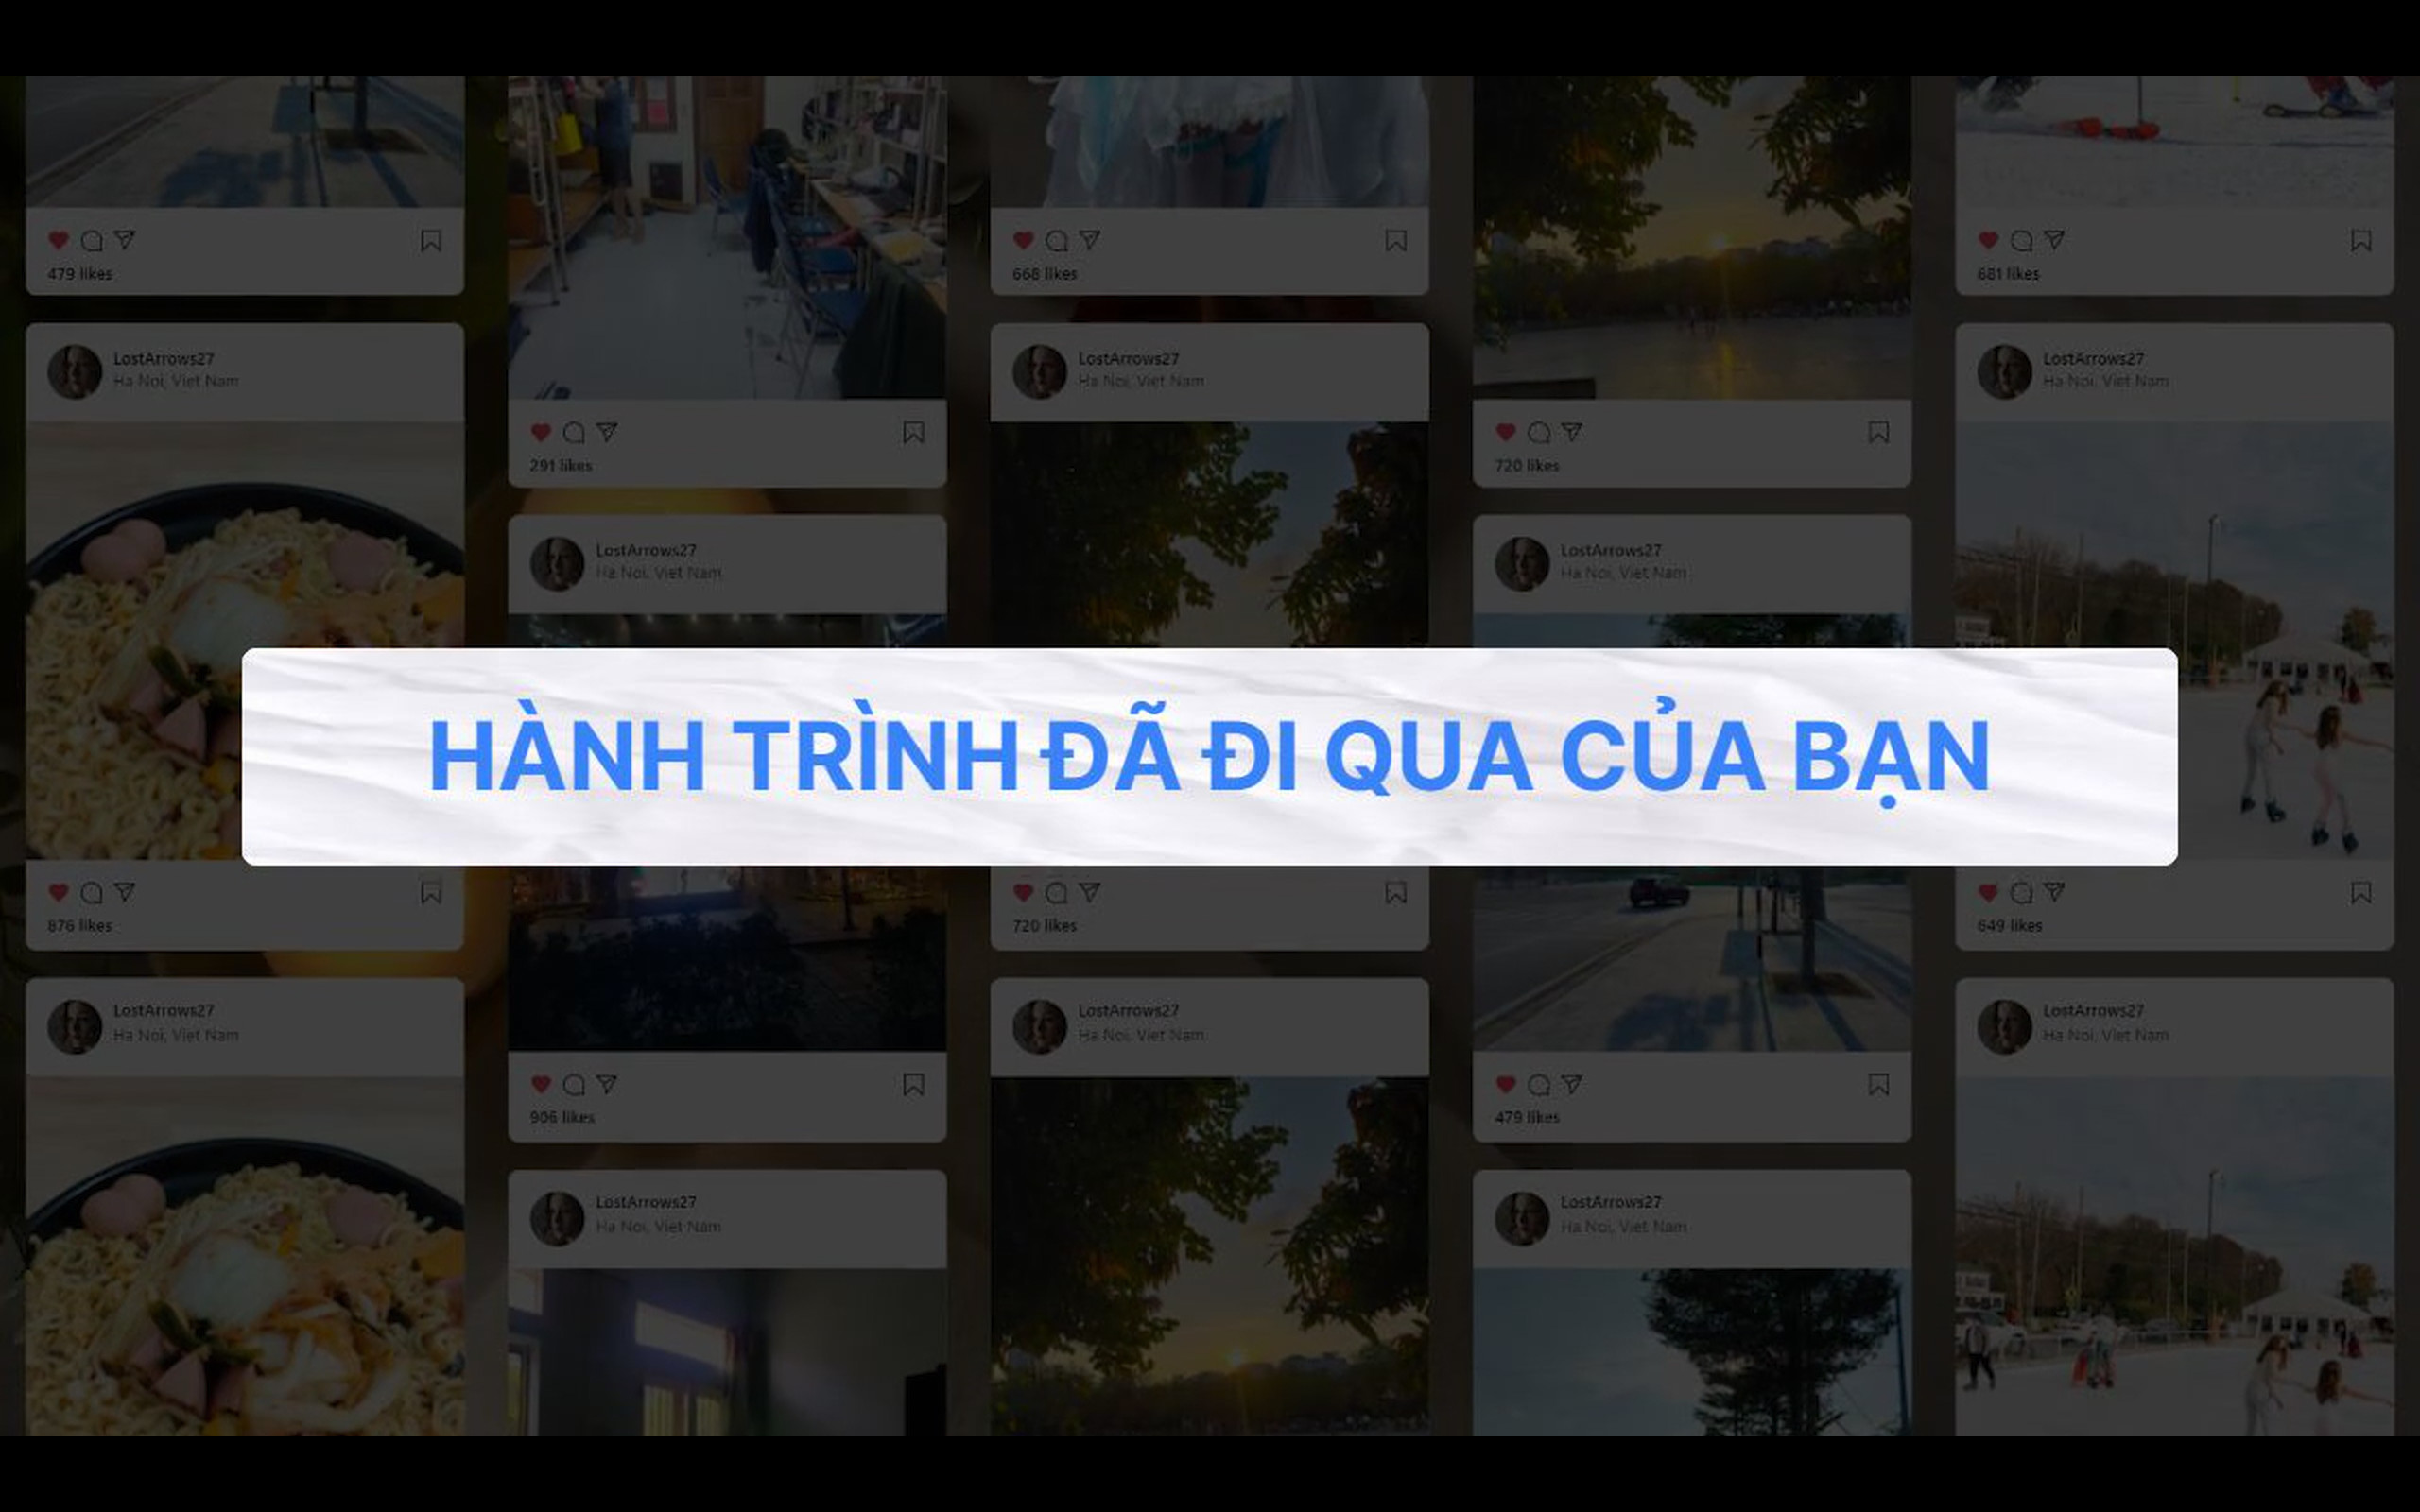
\includegraphics[width=1\linewidth]{figures/c4/4_1/intro_2.jpg} 
            \caption{Slide tổng quát video.}
        \end{subfigure}
        \caption{Các thiết kế cho phần Intro của video slideshow.}
        \label{fig:video-intro-design}
    \end{figure}
    
    \item \textbf{Content:}\newline
    Phần nội dung chính của video được tổ chức thành các chương (chapters), được phân chia dựa trên nhãn location và event của ảnh. Mỗi chương được cấu trúc bao gồm 1 slide tiêu đề và nhiều slide trình chiếu ảnh. Các slide trình chiếu ảnh được nhóm theo nhãn activity của ảnh. Cụ thể về cách phân chia các chương và slide sẽ được trình bày trong phần sau.
    
    Tiêu đề và caption của các khung hình được tạo tự động bằng mô hình Gemini thông qua prompt được trình bày trong hình \ref{fig:gemini-prompt} sau với input là các nhãn của ảnh trong chương đó:
    
    \begin{figure}[H]
        \centering  
        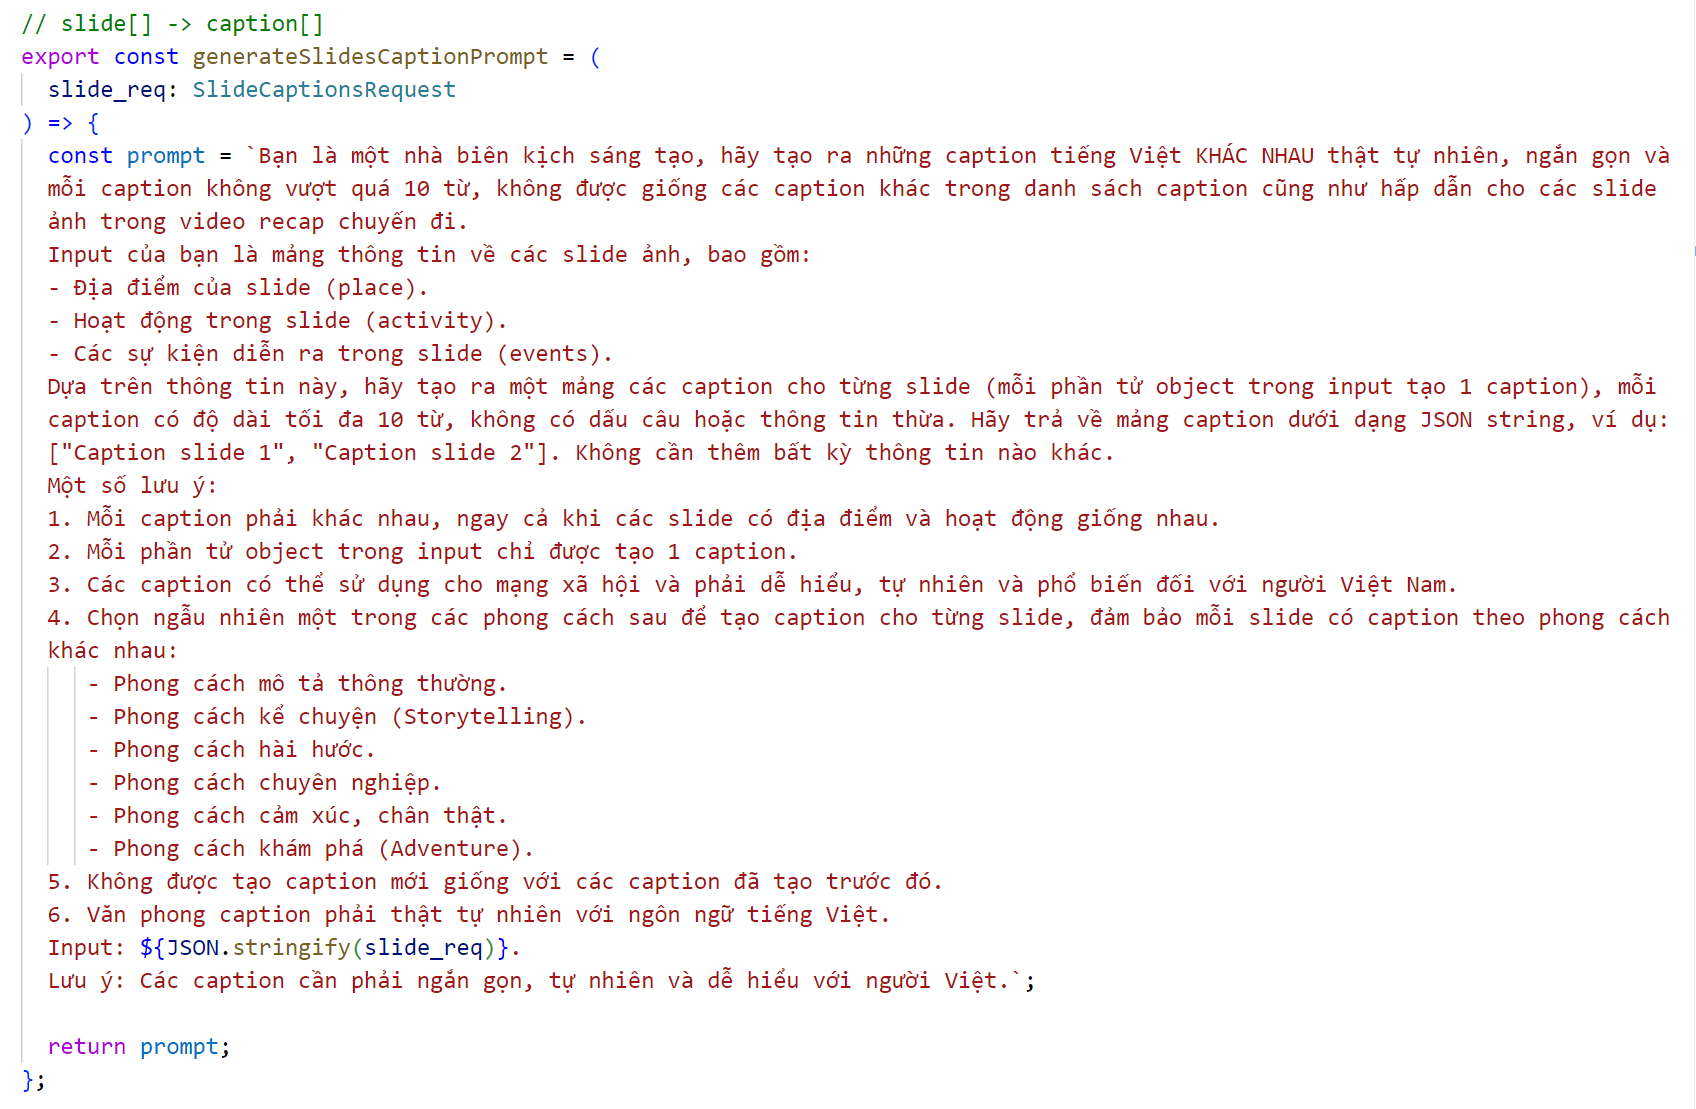
\includegraphics[width=0.82\textwidth]{figures/c4/4_1/prompt.png}
        \caption{Prompt Gemini để tạo caption cho video slideshow.}
        \label{fig:gemini-prompt}
    \end{figure}
    
    \newpage
    Ngoài ra, với mỗi chương, hệ thống đã chuẩn bị sẵn các phong cách trình bày sau cho slide ảnh:

    \begin{figure}[H]
        \centering
        % First row - Title styles
        \begin{subfigure}{0.48\textwidth}
            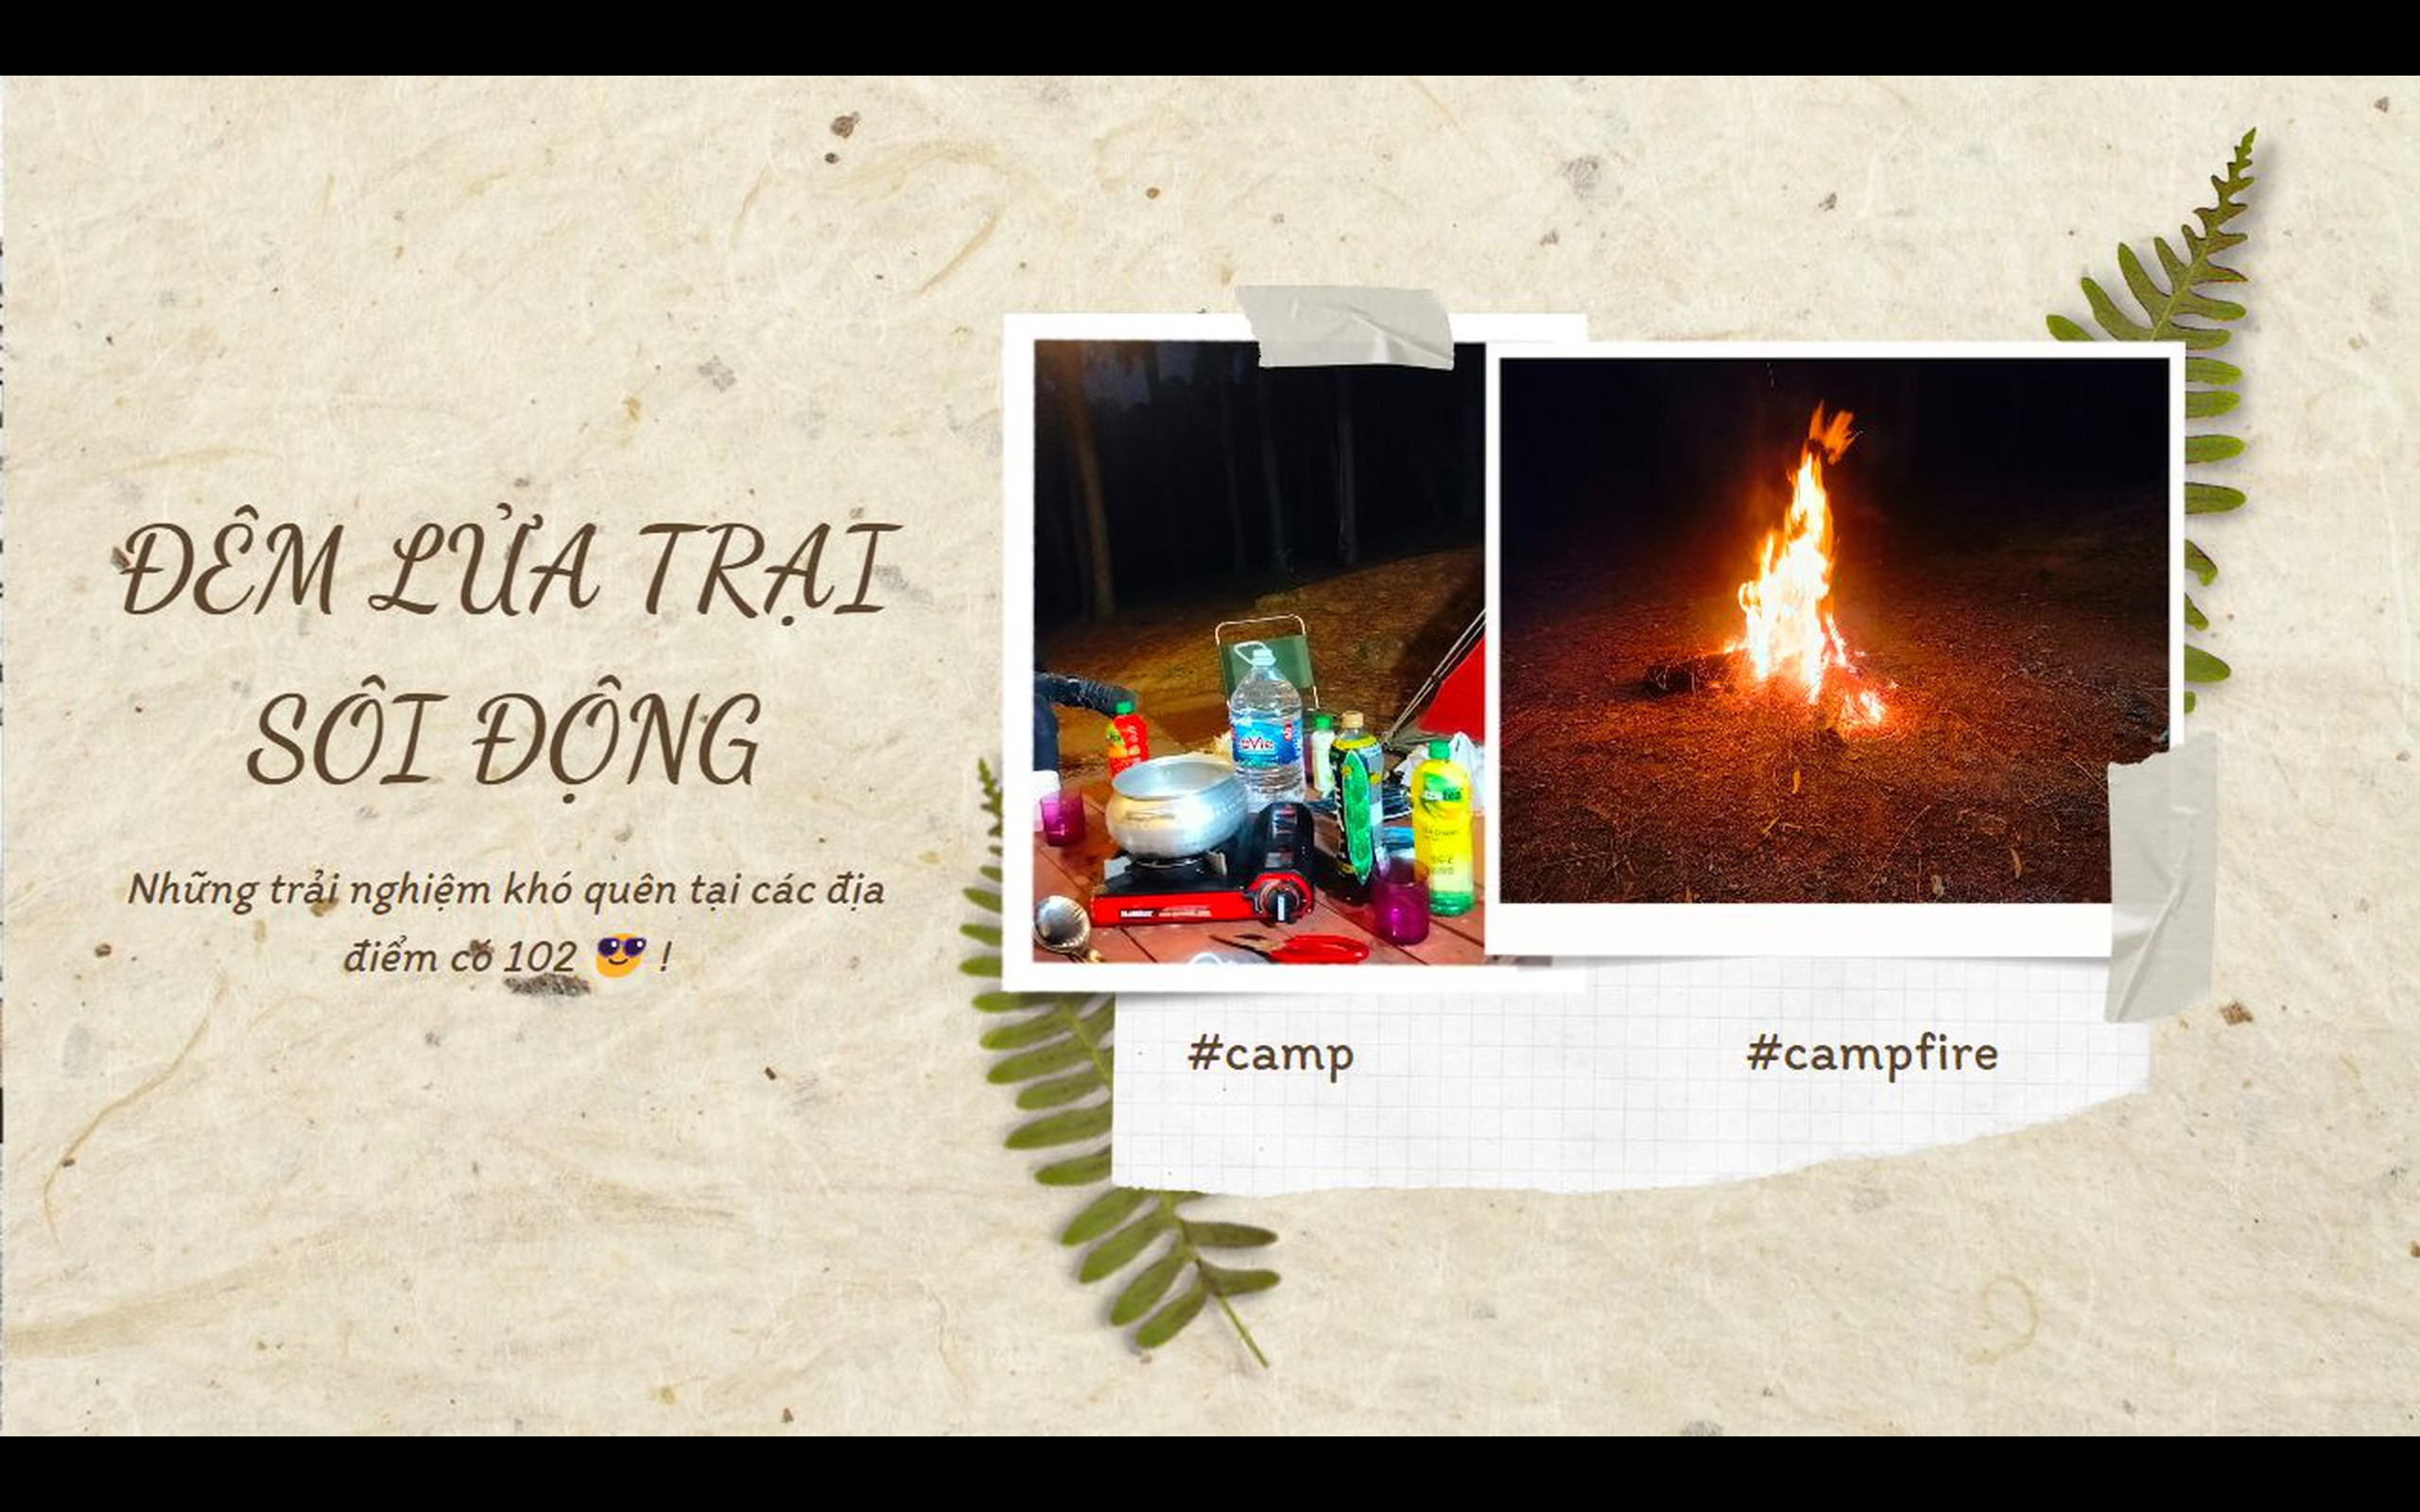
\includegraphics[width=1\linewidth]{figures/c4/4_1/title_1.jpg} 
            \caption{Style tiêu đề 1.}
        \end{subfigure}
        \hfill
        \begin{subfigure}{0.48\textwidth}
            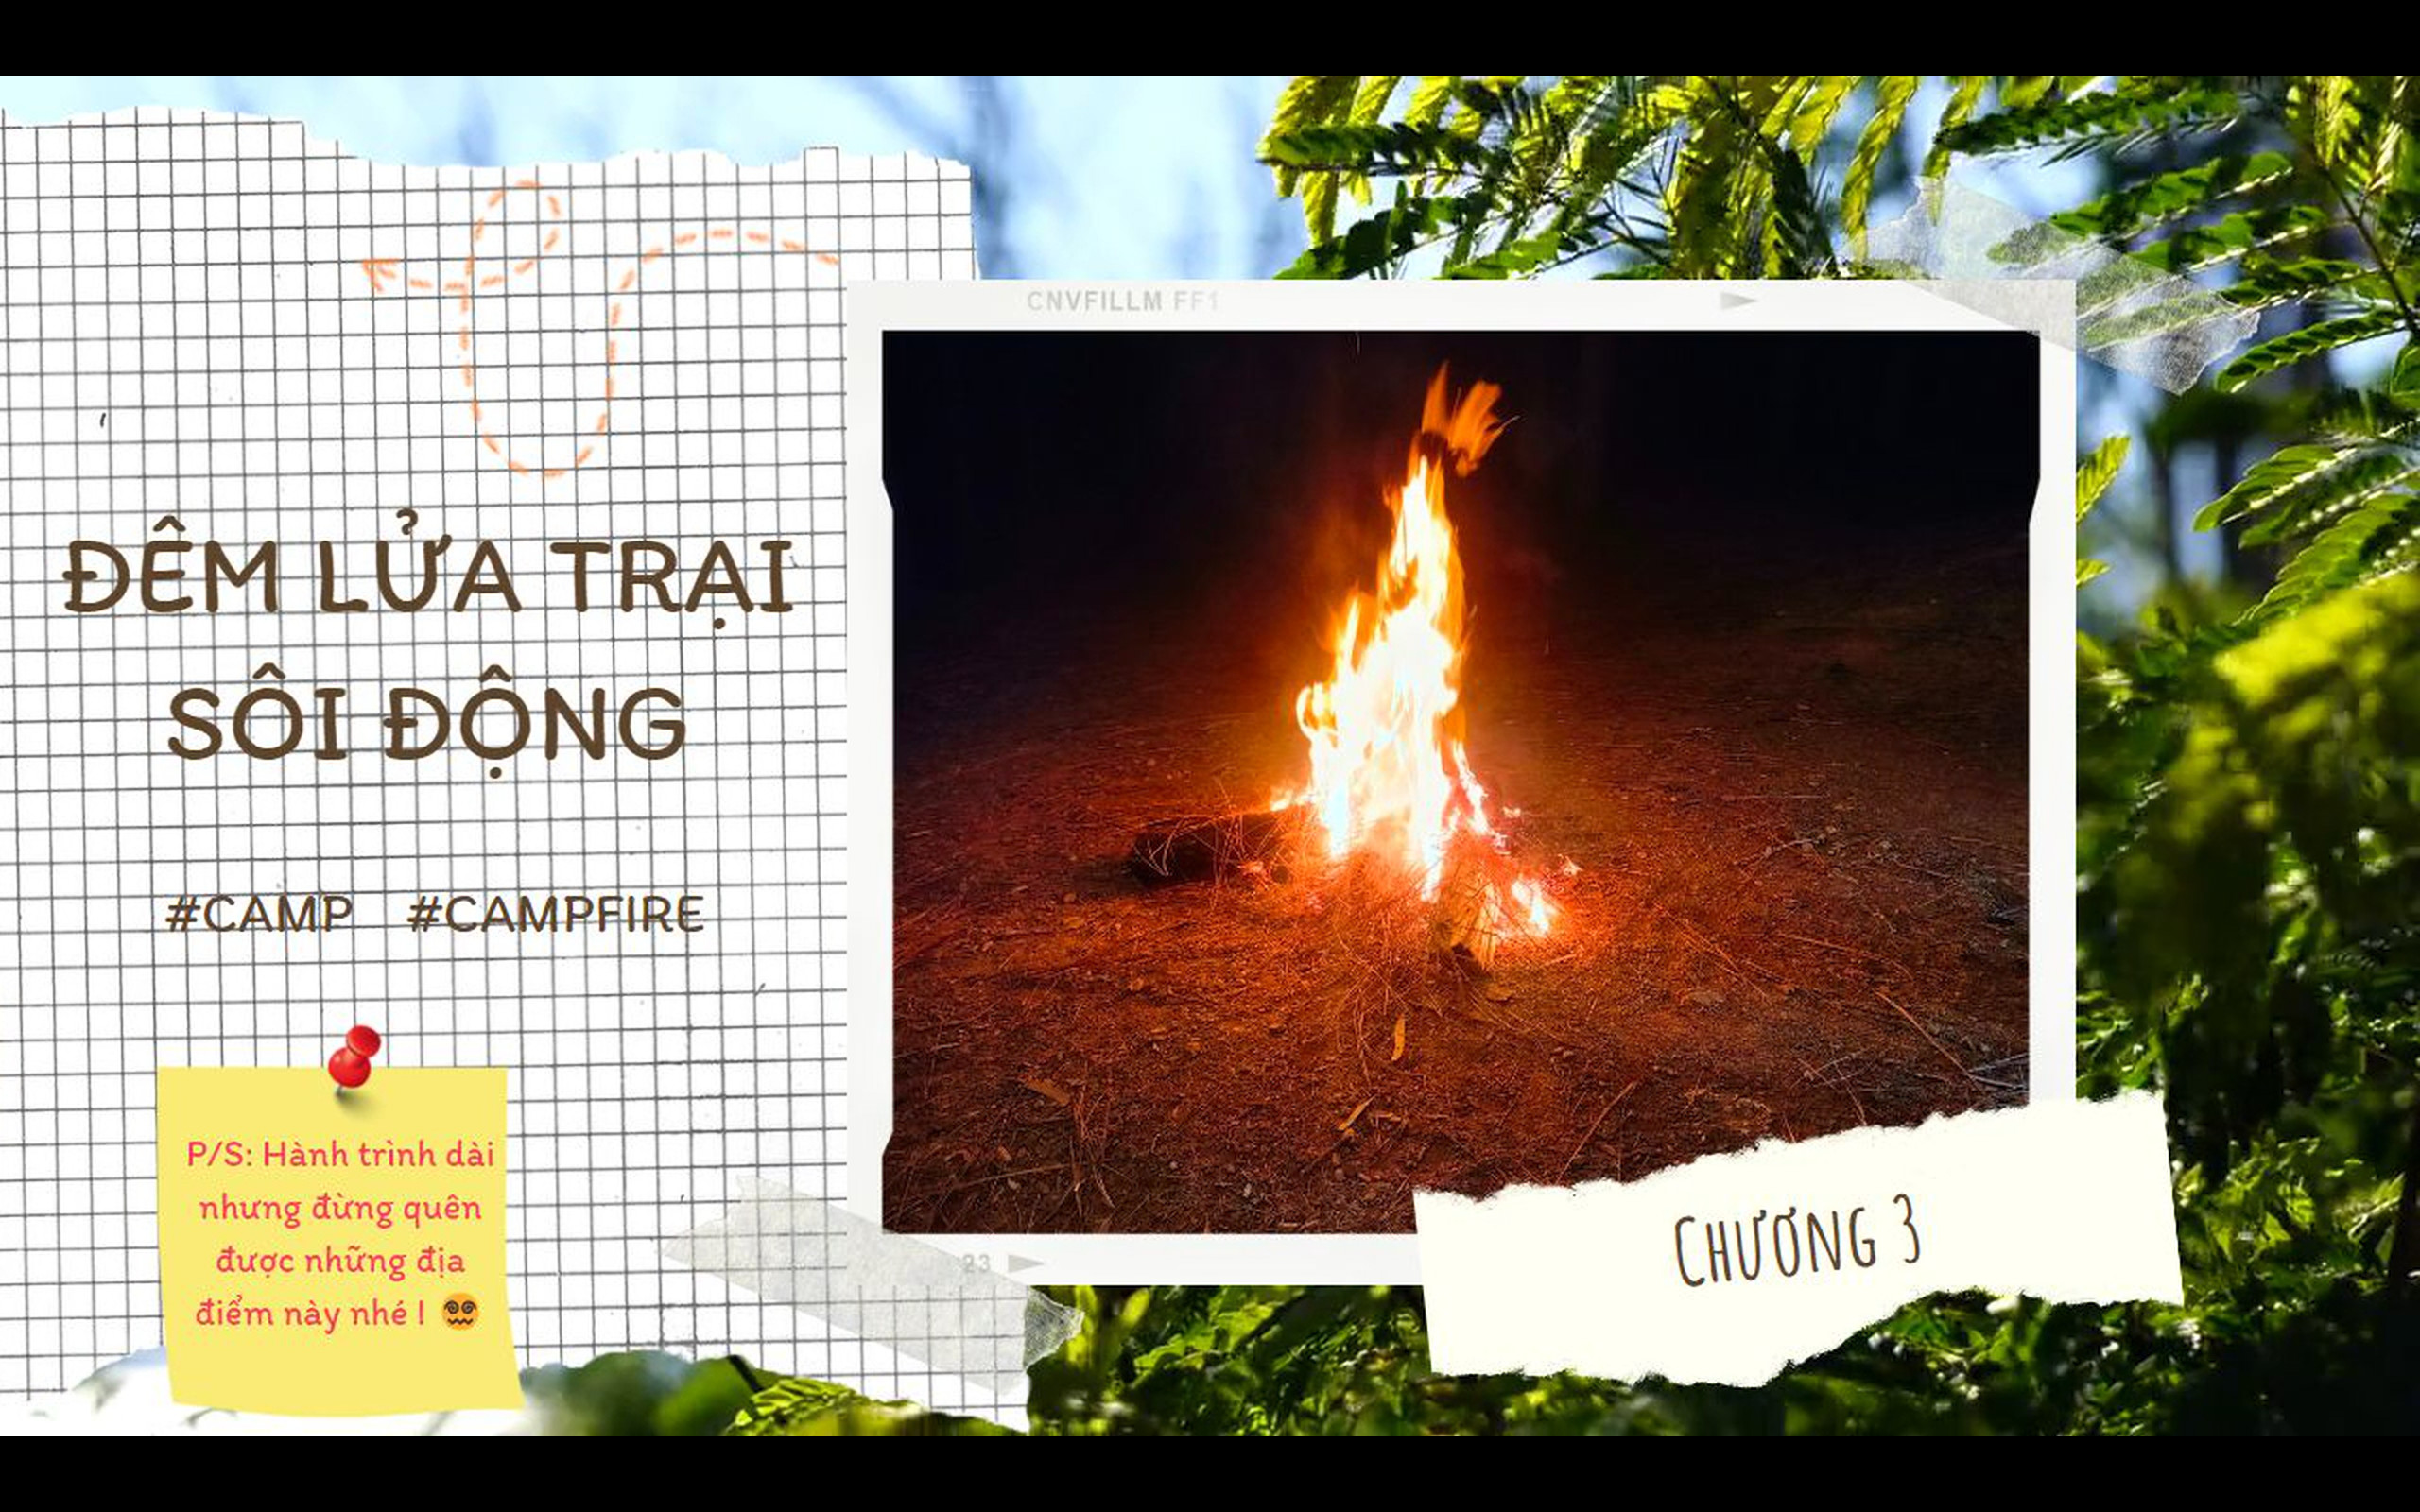
\includegraphics[width=1\linewidth]{figures/c4/4_1/title_2.jpg} 
            \caption{Style tiêu đề 2.}
        \end{subfigure}
        
        \vspace{0.5cm}
        % Second row - Slide styles
        \begin{subfigure}{0.48\textwidth}
            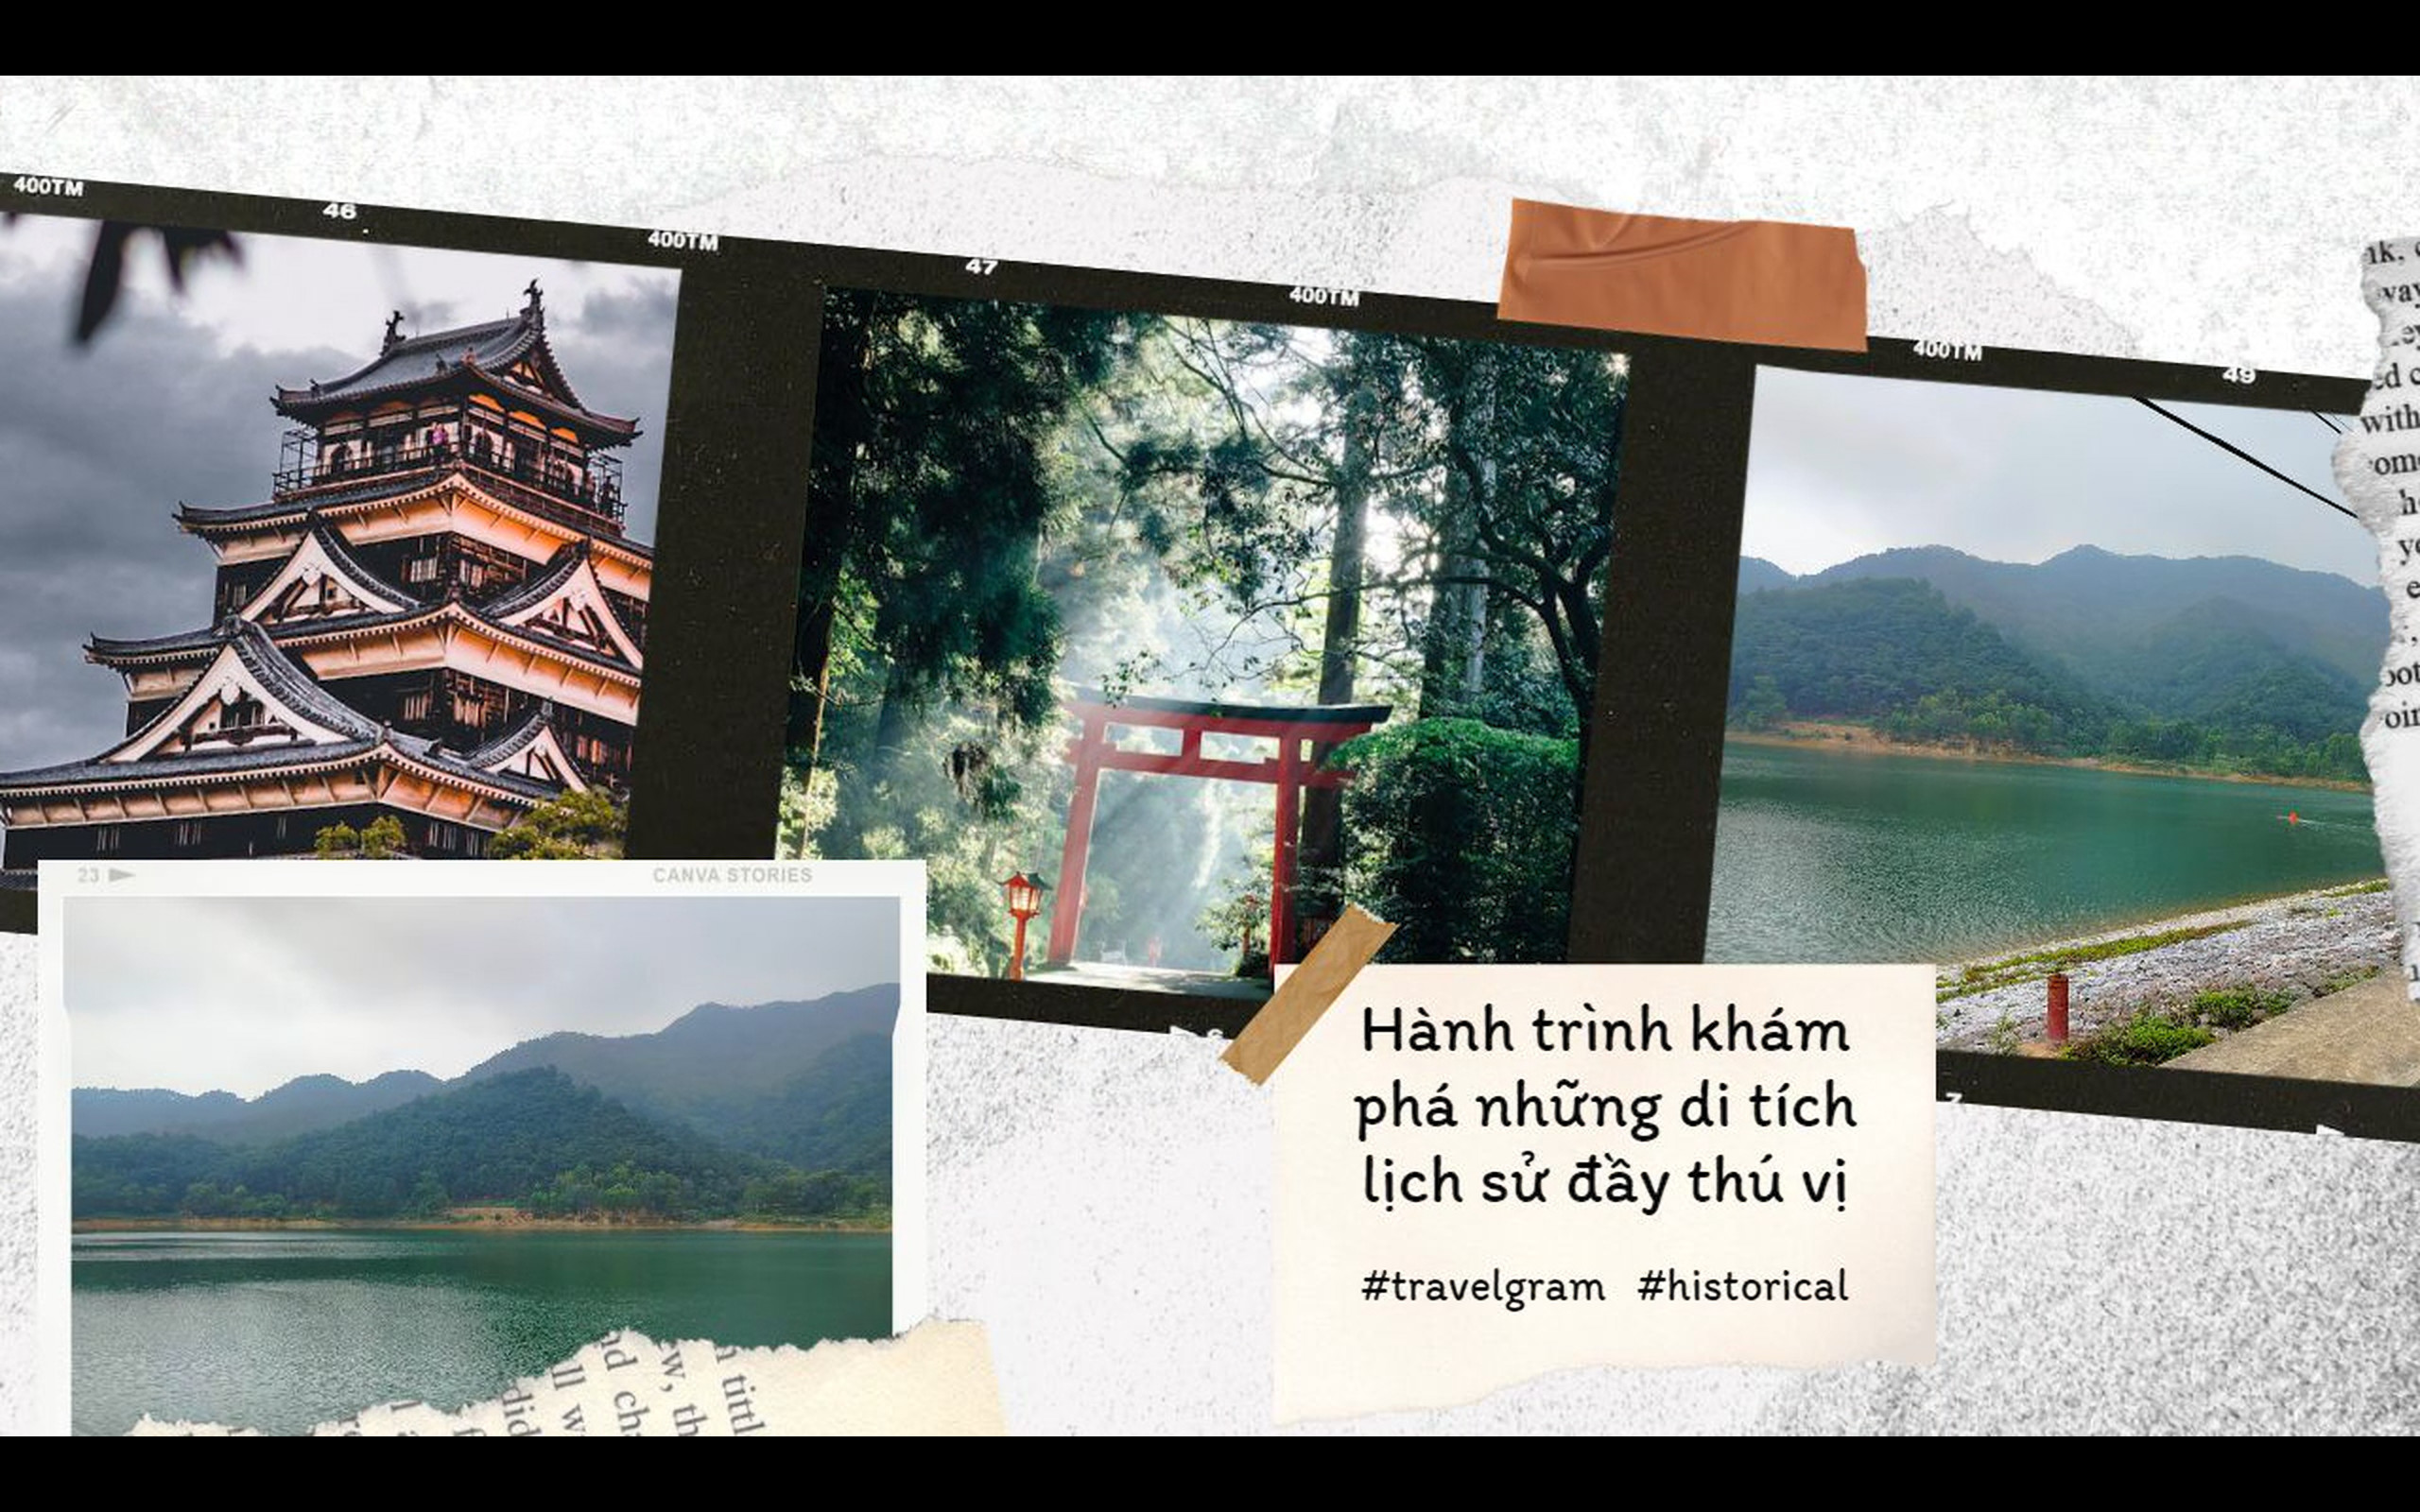
\includegraphics[width=1\linewidth]{figures/c4/4_1/slide_1.jpg} 
            \caption{Style slide ảnh 1.}
        \end{subfigure}
        \hfill
        \begin{subfigure}{0.48\textwidth}
            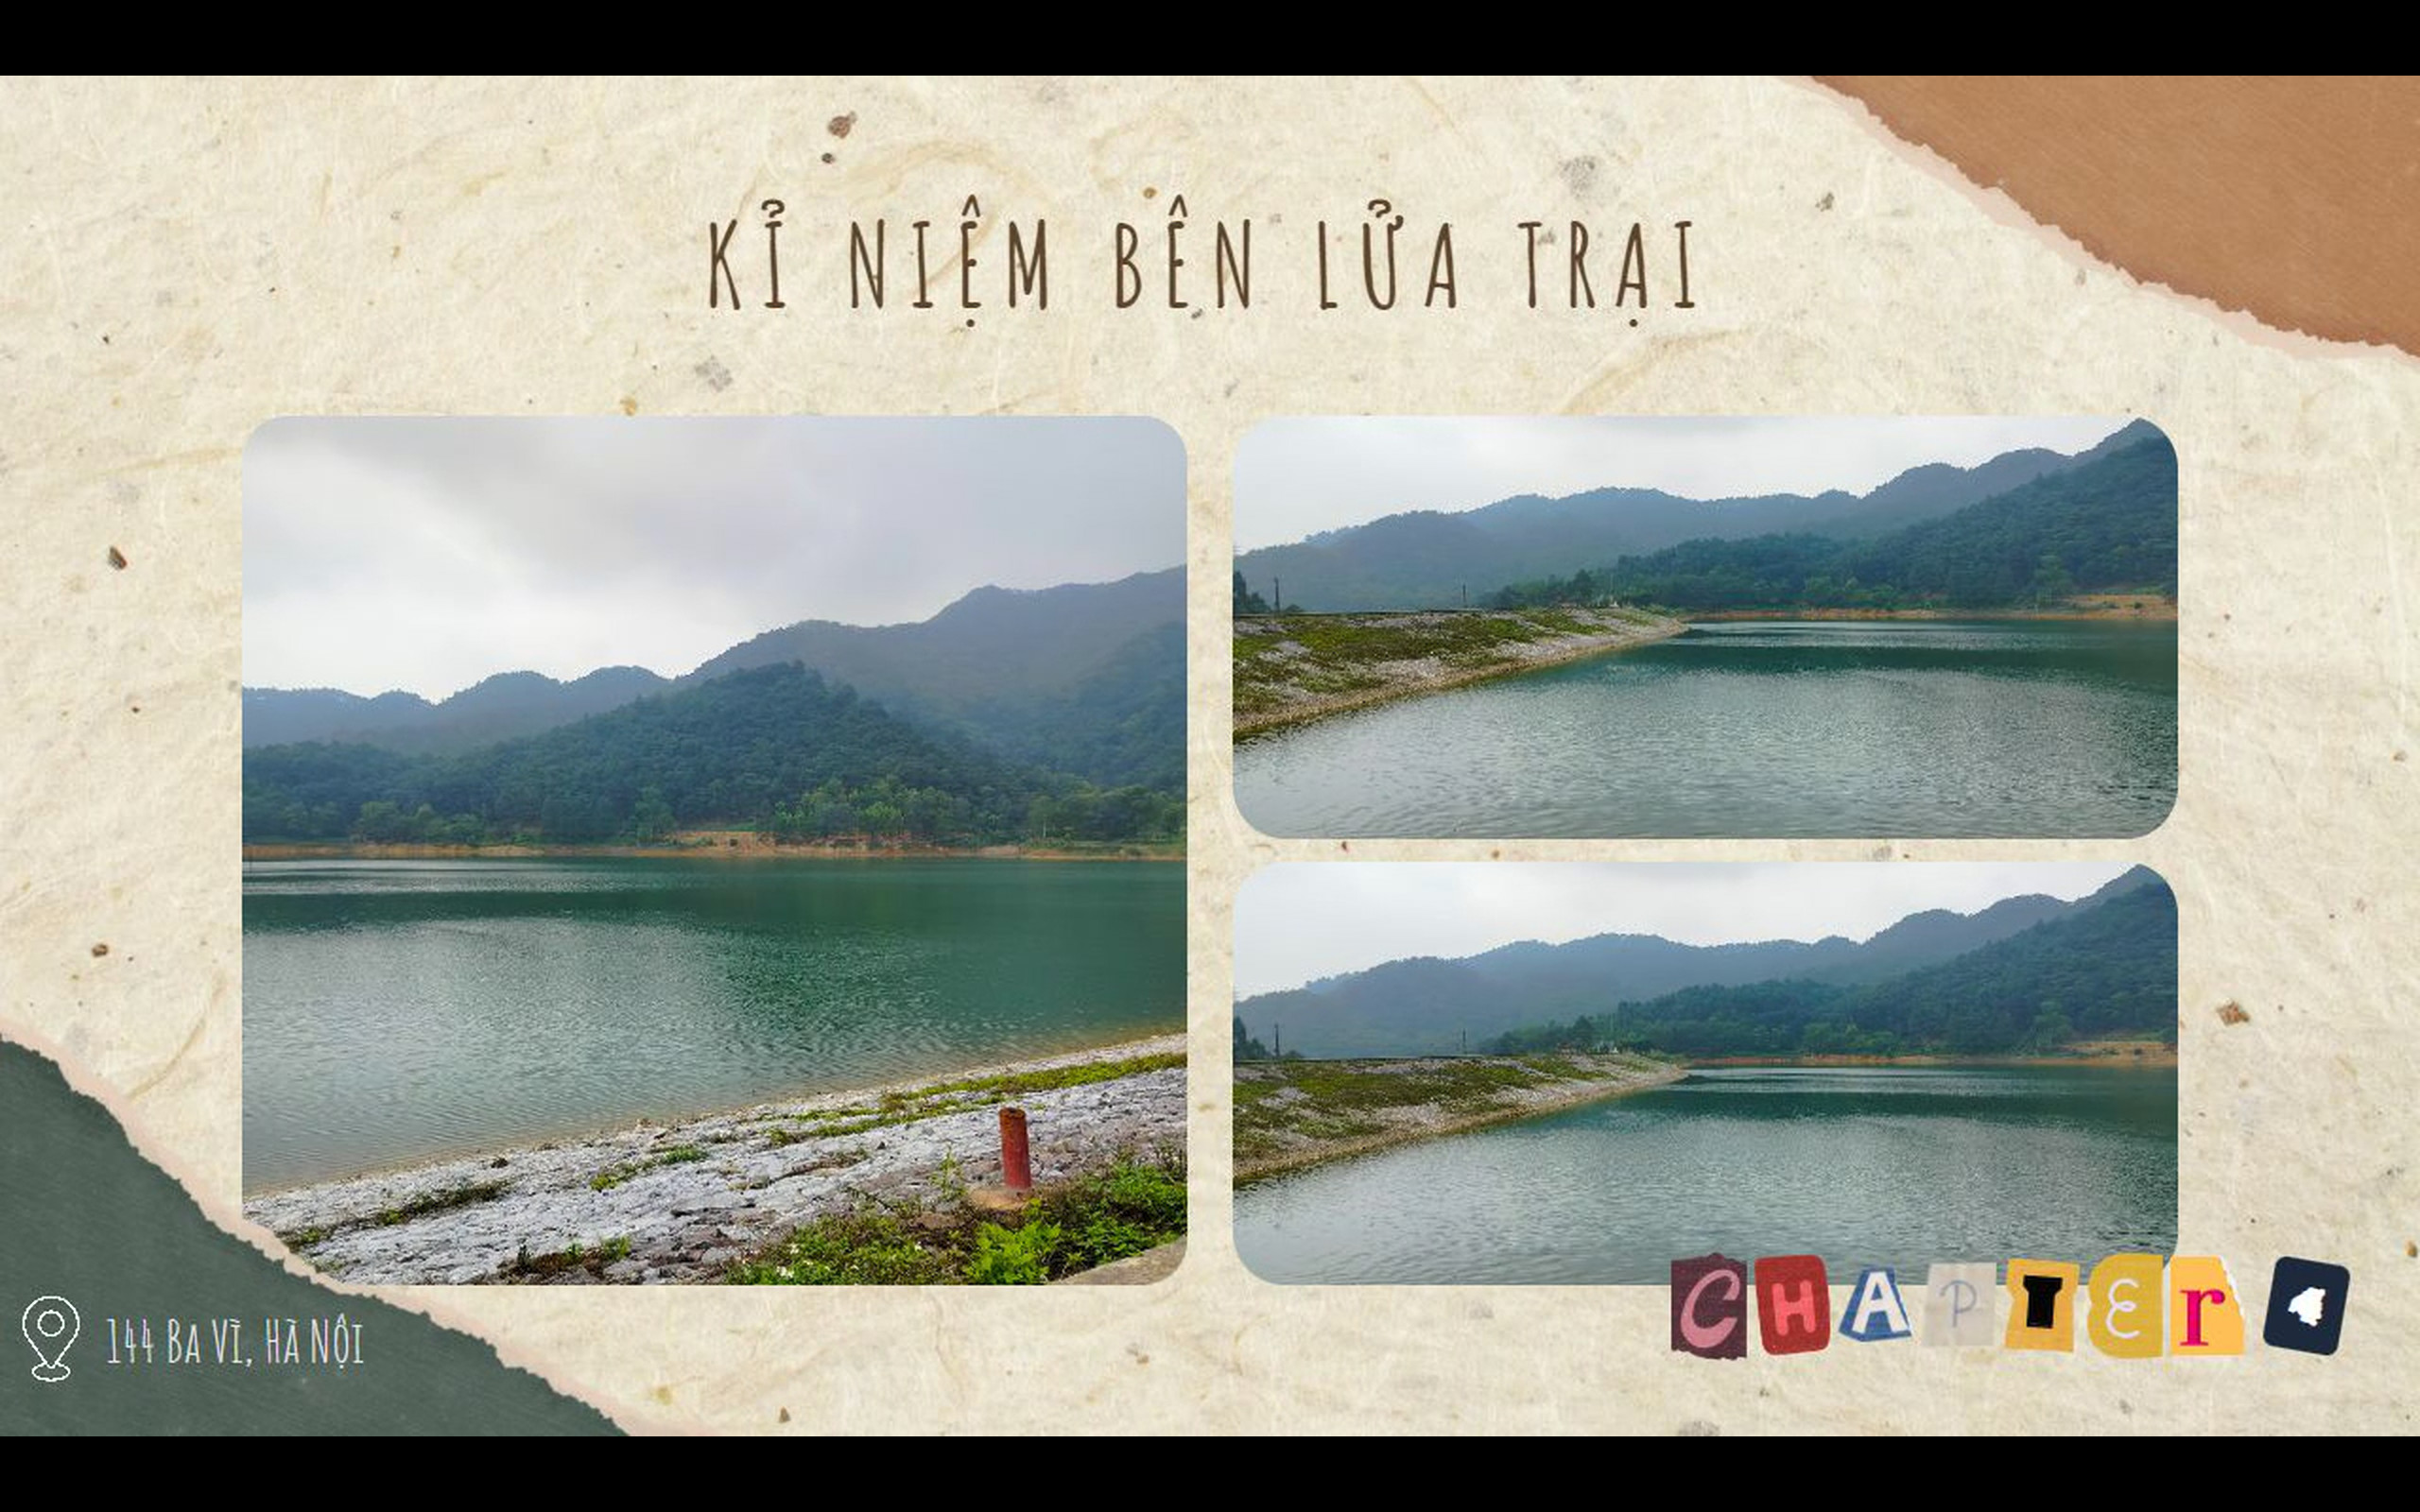
\includegraphics[width=1\linewidth]{figures/c4/4_1/slide_2.jpg} 
            \caption{Style slide ảnh 2.}
        \end{subfigure}
        
        \caption{Các style thiết kế cho tiêu đề chương và slide ảnh.}
        \label{fig:video-content-styles}
    \end{figure}
    
    \item \textbf{Special Part:}\newline
    Phần đặc biệt của video tập trung vào việc điểm lại các thành viên tham gia chuyến đi:
    \begin{itemize}
        \item[-] Chỉ xuất hiện khi bộ sưu tập có ít nhất một khuôn mặt được nhận diện.
        \item[-] Hiển thị tổng số người đã tham gia trong chuyến đi.
        \item[-] Trình bày top 4 khuôn mặt xuất hiện nhiều nhất cùng với tên của họ.
    \end{itemize}
    
    \begin{figure}[H]
        \centering
        \begin{subfigure}{0.48\textwidth}
            
\includegraphics[width=1\linewidth]{figures/c4/4_1/special_1.jpg} 
            \caption{Slide giới thiệu phần Special.}
        \end{subfigure}
        \hfill
        \begin{subfigure}{0.48\textwidth}
            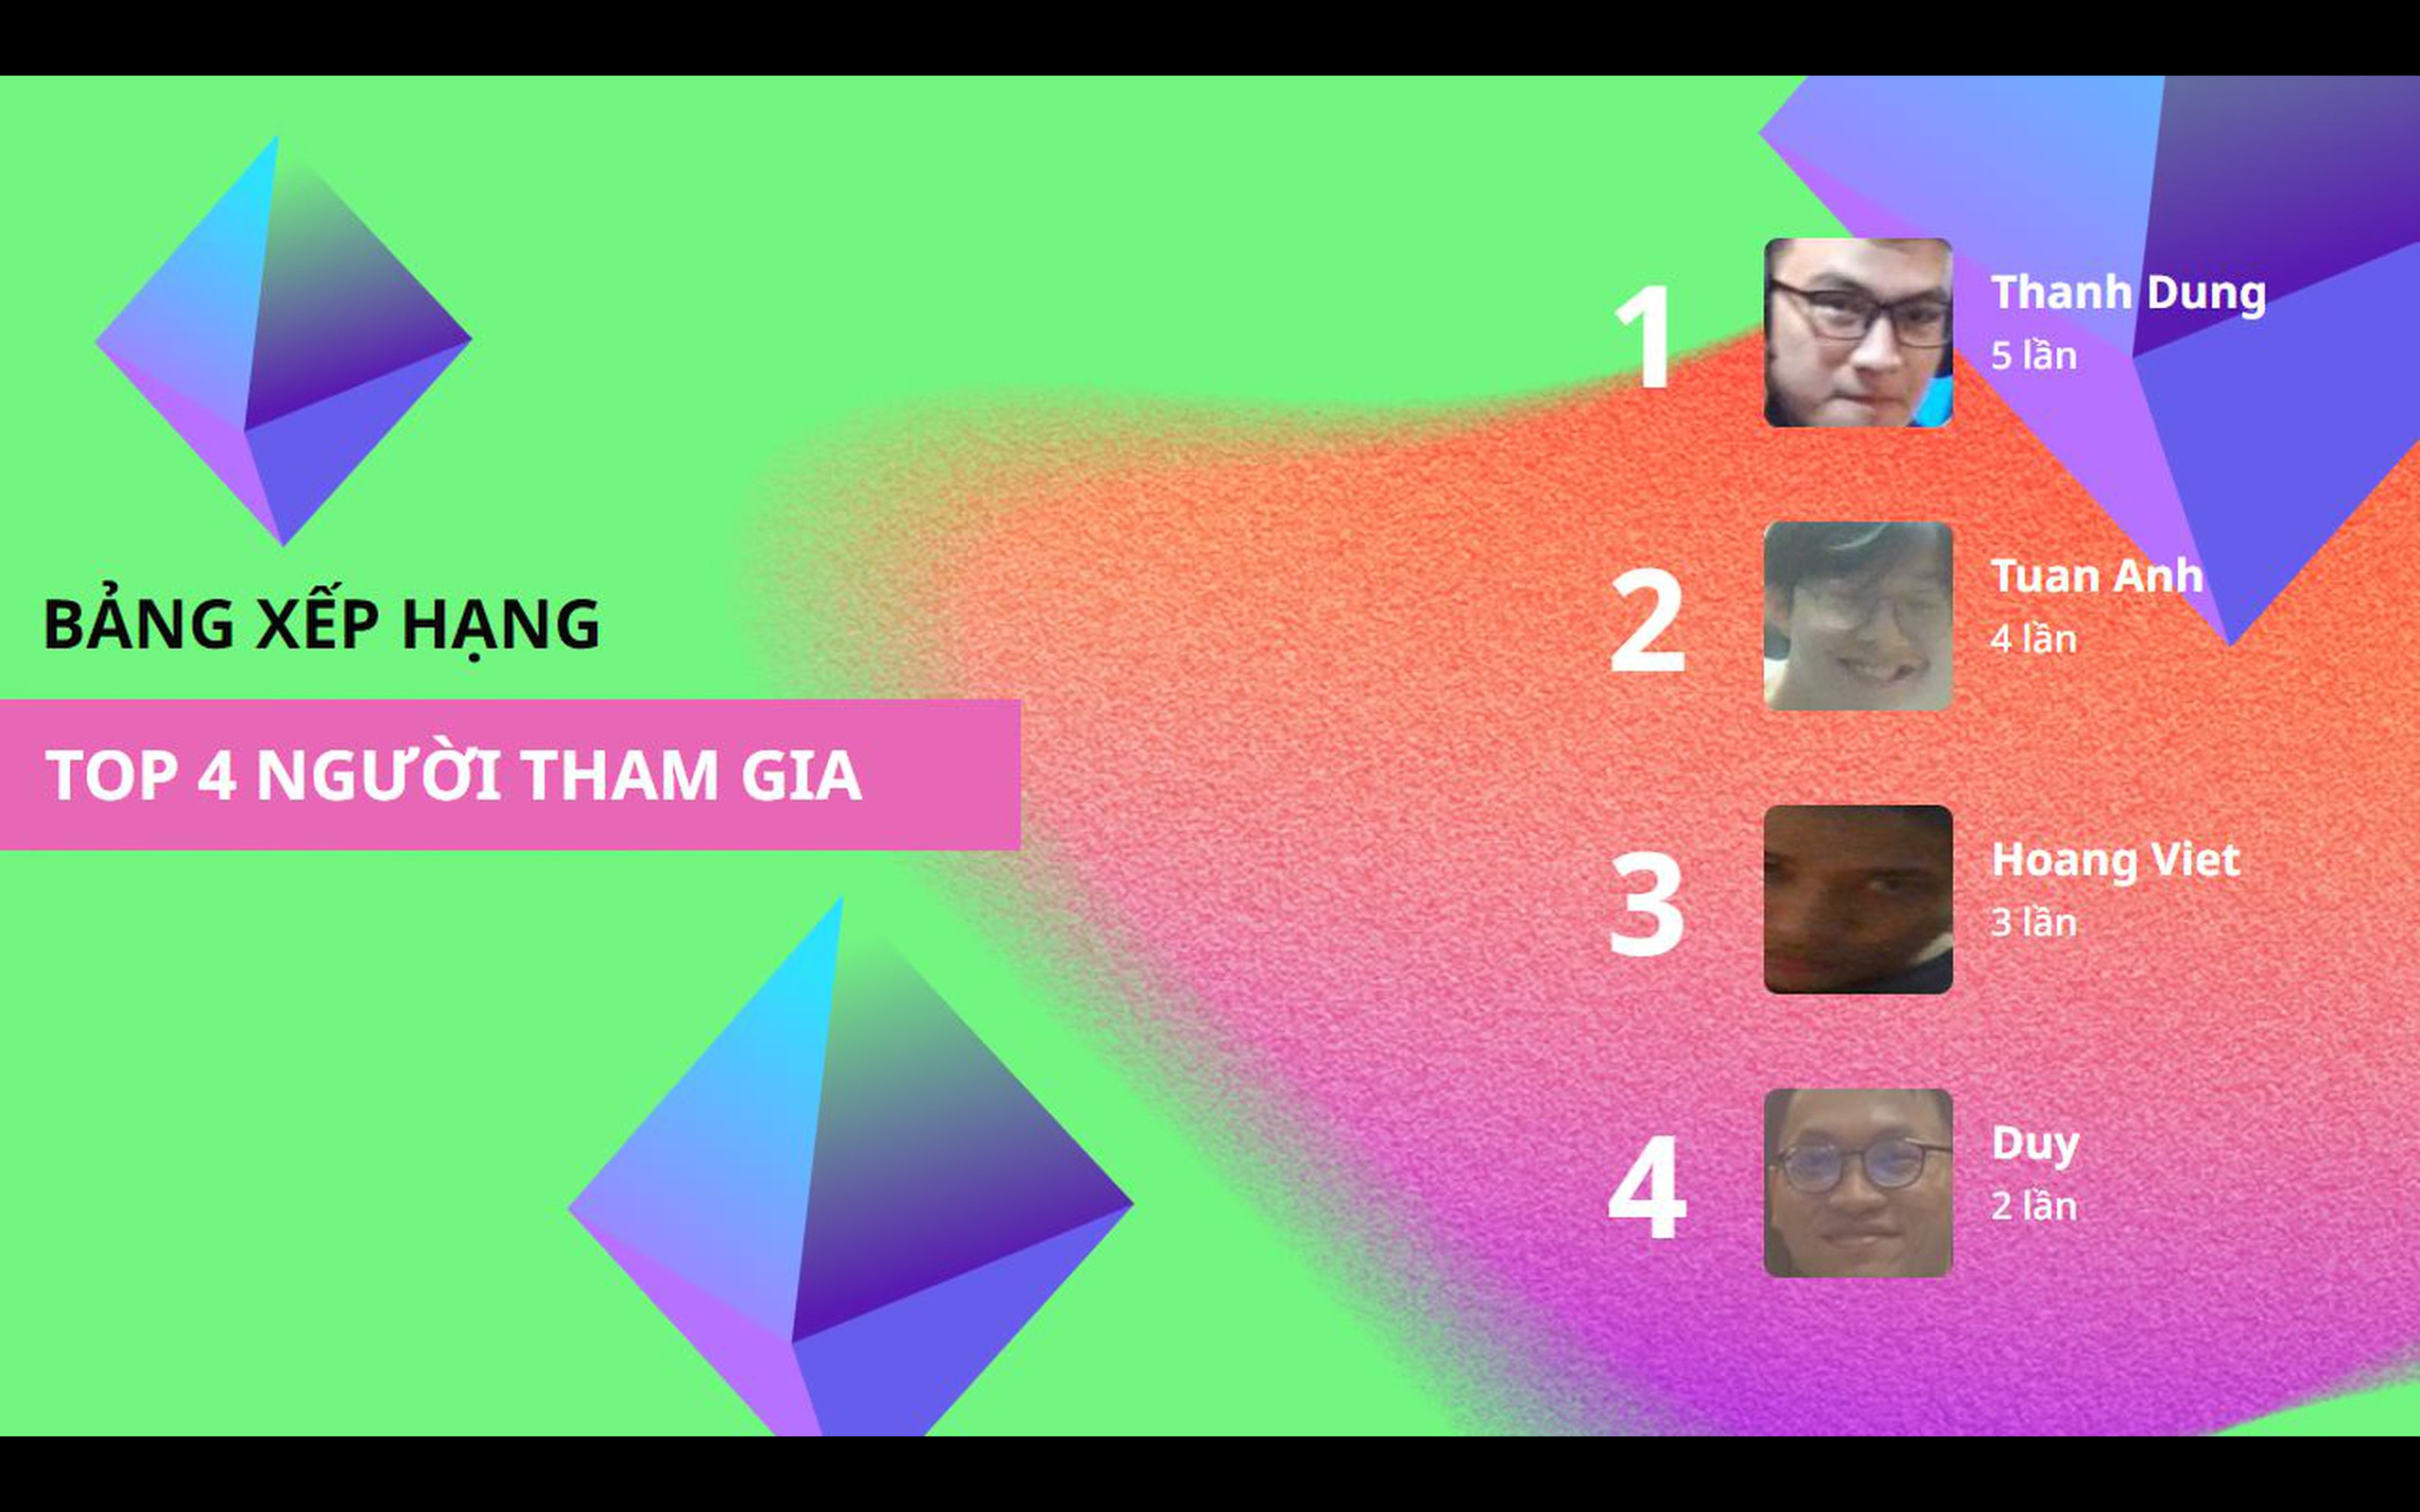
\includegraphics[width=1\linewidth]{figures/c4/4_1/special_2.jpg} 
            \caption{Slide hiển thị top khuôn mặt.}
        \end{subfigure}
        \caption{Thiết kế phần Special Part của video slideshow.}
        \label{fig:video-special-design}
    \end{figure}
    
    \item \textbf{Outro:}\newline
    Phần kết thúc của video sẽ tóm tắt lại chuyến đi bằng các ảnh tiêu biểu được chọn lọc và các caption được chọn tự động bởi hệ thống.
    
    \begin{figure}[H]
        \centering  
        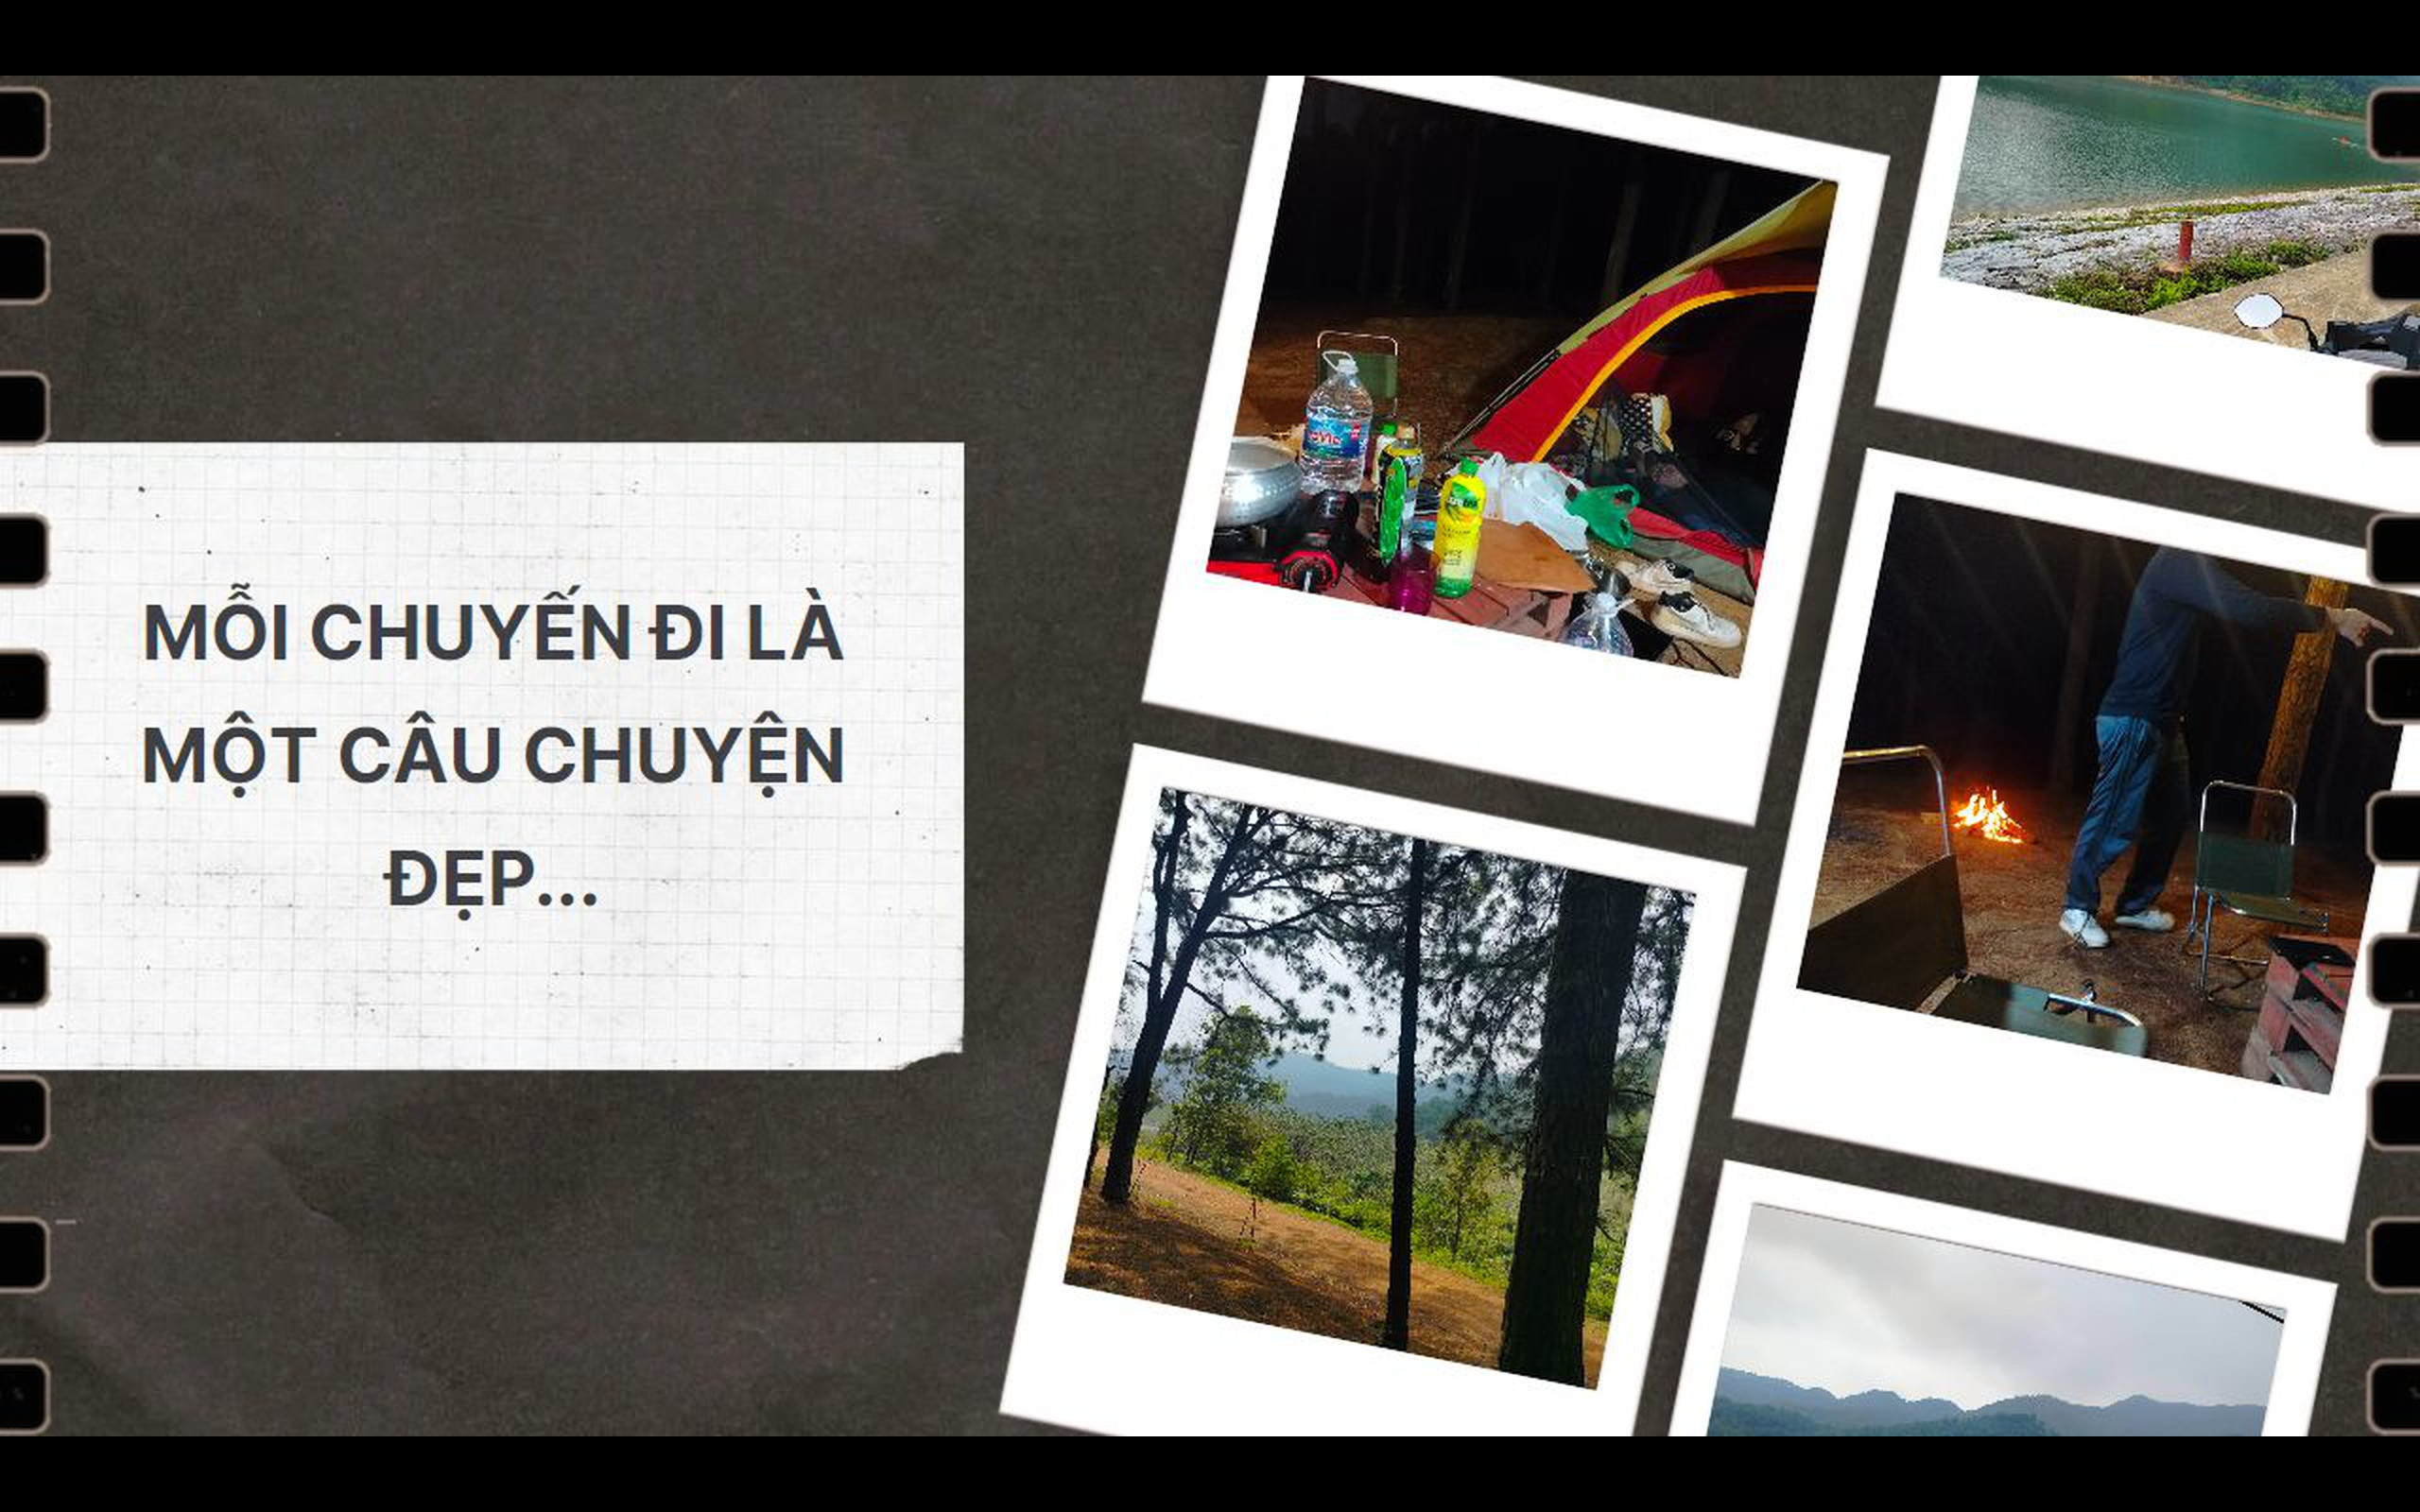
\includegraphics[width=1\textwidth]{figures/c4/4_1/outro.jpg}
        \caption{Thiết kế phần Outro của video slideshow.}
        \label{fig:video-outro-design}
    \end{figure}
\end{enumerate}

\paragraph{- Thuật toán xây dựng kịch bản (Content):}
Phần nội dung chính của video được xây dựng dựa trên thuật toán phân nhóm và tổ chức ảnh thành các chương dựa. Thuật toán này chia tập ảnh input của người dùng thành các nhóm dựa trên nhãn location và event của ảnh. Mỗi nhóm sẽ được tổ chức thành một chương riêng biệt trong video. Sau đây là cấu trúc JSON của label 1 ảnh mẫu với các nhãn location, action và event sau khi được phân loại bởi mô hình Open Clip:

\lstset{language=json}
\begin{lstlisting}[
    caption=Cấu trúc JSON của label ảnh,
    label=lst:json-label,
    captionpos=t,
    belowcaptionskip=20pt]
{
  "location_labels": [
    {"temple": 0.9948057532310486},
    {"palace": 0.0011160931317135692}
  ],
  "action_labels": [
    {"visiting historical sites": 0.8663983941078186},
    {"visiting museum": 0.039322637021541595}
  ],
  "event_labels": [
    {"Spring": 0.3410003185272217},
    {"Conference": 0.1293141394853592}
  ]
}
\end{lstlisting}

Quy trình tạo kịch bản phần Content (nội dung chính) của video bao các bước chính sau:

\begin{itemize}
    \item \textbf{Bước 1 - Labeling}: Phát hiện và gán nhãn cho những ảnh chưa có nhãn. Khi đó, hệ thống sẽ gửi yêu cầu phân loại ảnh đến server labeling ảnh. 
    
    \item \textbf{Bước 2 - Nhóm ảnh theo nhãn}: Nhóm các ảnh theo nhãn địa điểm có độ tin cậy (\%) cao nhất của từng ảnh. Kết quả phân loại sẽ gồm các nhóm chứa các ảnh có nhãn địa điểm giống nhau
    Ví dụ: \{mountain: 2 ảnh\}, \{park: 3 ảnh\}.
    
    \item \textbf{Bước 3 - Nhóm theo tập nhãn rộng hơn}: Các nhóm có số lượng ảnh < 3 sẽ được nhóm chung dựa theo tập nhãn rộng hơn. Tập nhãn rộng hơn (broader group) là tập hợp các nhãn địa điểm (location) được phân loại vào các nhóm lớn hơn (như ``nature'' bao gồm ``sea'', ``mountain'', ``forest'', v.v.). Ví dụ kết quả phân loại bước 3: nếu nhóm ``sea'' có 2 ảnh và nhóm ``mountain'' có 2 ảnh, cả hai sẽ được gộp thành nhóm ``nature'' với 4 ảnh.
    
    \item \textbf{Bước 4 - Tối ưu hóa nhóm}: Kiểm tra lại các nhóm ``broader group'' có số lượng < 3 ảnh. Nếu phát hiện, hệ thống sẽ đưa nhóm này vào nhóm địa điểm thuộc ``broader location'' đó và có số lượng ảnh nhiều nhất. Ví dụ: nhóm ``workspace'' (gồm 2 ảnh) sẽ được gộp vào nhóm ``classroom'' (có 4 ảnh) nếu ``classroom'' thuộc nhóm rộng hơn có tên ``workspace'' và có số lượng ảnh nhiều nhất trong các nhóm địa điểm thuộc ``workspace''.
     
    \item \textbf{Bước 5 - Xử lý ngoại lệ}: Duyệt lại lần cuối, những nhóm chỉ có 1 ảnh sẽ được gộp vào một nhóm chung và hiển thị dưới dạng 1 chương đặc biệt có tên là ``Small Part'' hoặc ``Khoảnh khắc khác''.
    \item \textbf{Bước 6 - Tạo nội dung từng chương}: Trong các chương, với tập ảnh đã được nhóm và phân chia từ các bước trước, hệ thống sẽ tạo tiêu đề chương và chia các ảnh trong chương đó thành các slide ảnh. Mỗi slide ảnh được nhóm theo nhãn hoạt động (activity). 
    \item \textbf{Bước 7 - Tạo tiêu đề và caption}: Tiêu đề chương và caption được tạo tự động bằng mô hình Gemini thông qua prompt đã nêu ở trên. 
    \item \textbf{Bước 8 - Chọn phong cách trình bày}: Hệ thống sẽ chọn ngẫu nhiên một trong các phong cách trình bày đã được chuẩn bị sẵn cho tiêu đề chương và slide ảnh (nếu người dùng không chọn phong cách cụ thể nào).
    \item \textbf{Bước 9 - Nhóm khuôn mặt}: Hệ thống sẽ lấy dữ liệu các nhóm khuôn mặt trong CSDL của người dùng và chọn ra 4 nhóm khuôn mặt có số lượng ảnh lớn nhất để hiển thị trong phần Đặc biệt (Special Part) của video. Nếu không có khuôn mặt nào được nhận diện, phần này sẽ không được hiển thị.
\end{itemize}

\paragraph{- Lưu trữ kịch bản video:}
Sau khi được xây dựng hoàn chỉnh, kịch bản video được lưu trữ vào cơ sở dữ liệu trong bảng \texttt{video\_render}, cụ thể là trong trường \texttt{schema}. Thông tin này sau đó được sử dụng bởi các module render video để tạo ra video slideshow hoàn chỉnh theo kịch bản đã định. Ngoài ra, việc lưu trữ kịch bản cho phép hệ thống:
\begin{itemize}
    \item[-] Xem lại và chỉnh sửa kịch bản trước khi render nếu cần
    \item[-] Tái sử dụng kịch bản cho các video khác với cùng bộ ảnh
    \item[-] Theo dõi và phân tích các mẫu kịch bản phổ biến để cải thiện thuật toán
\end{itemize}

\subsubsection{Tạo video slideshow}
Video sẽ được hệ thống render dựa trên kịch bản đã lưu trong CSDL thông qua những bước sau:

\begin{enumerate}
    \item \textbf{Lấy kịch bản video}: Hệ thống sẽ truy vấn kịch bản video từ bảng \texttt{video\_render} trong cơ sở dữ liệu.
    \item \textbf{Tối ưu hóa render}: Trong quá trình thử nghiệm và đo đạc thời gian tạo video, hệ thống bị treo khá lâu do thời gian render video ở phần Intro. Vì vậy thời gian render đã được tối ưu bằng cách upload và resize ảnh của video bằng server của Cloudinary~\cite{cloudinary}. Do hạn chế về dung lượng upload của Cloudinary, hiện tại phần tối ưu hóa render sẽ chỉ được hệ thống áp dụng cho phần Mở đầu (Intro) của video.
    \item \textbf{Ghép kịch bản video}: Hệ thống ghép các yếu tố trong kịch bản video vào các khung hình (frame) được lập trình sẵn. Các yếu tố này bao gồm: ảnh, tiêu đề chương, caption, hiệu ứng chuyển cảnh, âm thanh nền và các yếu tố khác.
    \item \textbf{Render video}: Hệ thống sẽ sử dụng thư viện Remotion để tạo video định dạng mp4 với các khung hình và kịch bản đã lưu. Sau đó lưu video vào 1 thư mục tạm thời trên server. Trong quá trình render, hệ thống sẽ lưu trạng thái tạo video của người dùng vào trong CSDL Redis để tránh tình trạng người dùng tạo nhiều video 1 lúc, qua đó giảm tải cho server.
    \item \textbf{Tối ưu hóa video cho quá trình streaming}: Sau khi đã hoàn thành video, hệ thống sẽ sử dụng thư viện ffmpeg để chuyển đổi định dạng video sang m3u8, giúp tối ưu hóa cho quá trình streaming video trên ứng dụng. 
    \item \textbf{Lưu video vào CSDL}: Video sau khi được tối ưu hóa sẽ được lưu vào bảng \texttt{video\_chunk} trong cơ sở dữ liệu.
\end{enumerate}

